% Created by tikzDevice version 0.12.3.1 on 2022-09-05 13:27:06
% !TEX encoding = UTF-8 Unicode
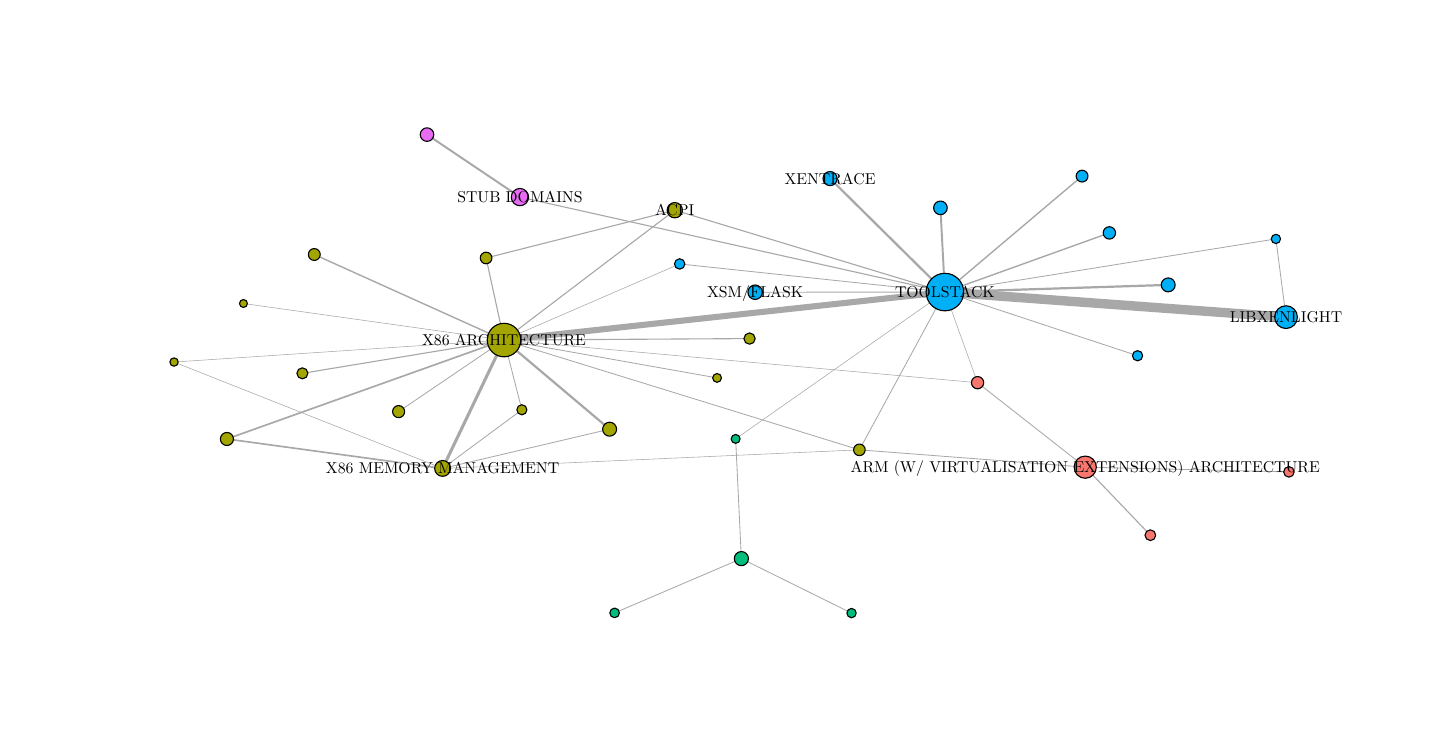
\begin{tikzpicture}[x=1pt,y=1pt]
\definecolor{fillColor}{RGB}{255,255,255}
\path[use as bounding box,fill=fillColor,fill opacity=0.00] (0,0) rectangle (505.89,252.94);
\begin{scope}
\path[clip] (  0.00,  0.00) rectangle (505.89,252.94);
\definecolor{fillColor}{RGB}{255,255,255}

\path[fill=fillColor] (  0.00,  0.00) rectangle (505.89,252.94);
\end{scope}
\begin{scope}
\path[clip] ( 32.75, 32.75) rectangle (475.89,222.94);
\definecolor{drawColor}{gray}{0.66}

\path[draw=drawColor,line width= 0.4pt,line join=round] (233.84,186.98) -- (165.65,169.72);

\path[draw=drawColor,line width= 0.4pt,line join=round] (233.84,186.98) -- (331.43,157.40);

\path[draw=drawColor,line width= 0.4pt,line join=round] (233.84,186.98) -- (172.12,140.06);

\path[draw=drawColor,line width= 0.5pt,line join=round] (103.57,170.97) -- (172.12,140.06);

\path[draw=drawColor,line width= 0.3pt,line join=round] (255.82,104.34) -- (257.89, 61.08);

\path[draw=drawColor,line width= 0.2pt,line join=round] (255.82,104.34) -- (331.43,157.40);

\path[draw=drawColor,line width= 0.4pt,line join=round] (382.15, 94.13) -- (405.68, 69.54);

\path[draw=drawColor,line width= 0.3pt,line join=round] (382.15, 94.13) -- (343.24,124.65);

\path[draw=drawColor,line width= 0.3pt,line join=round] (382.15, 94.13) -- (455.75, 92.43);

\path[draw=drawColor,line width= 0.3pt,line join=round] (382.15, 94.13) -- (300.54,100.39);

\path[draw=drawColor,line width= 0.3pt,line join=round] (297.70, 41.40) -- (257.89, 61.08);

\path[draw=drawColor,line width= 0.3pt,line join=round] (134.04,114.20) -- (172.12,140.06);

\path[draw=drawColor,line width= 0.3pt,line join=round] (235.60,167.56) -- (331.43,157.40);

\path[draw=drawColor,line width= 0.2pt,line join=round] (235.60,167.56) -- (172.12,140.06);

\path[draw=drawColor,line width= 0.5pt,line join=round] (390.87,178.78) -- (331.43,157.40);

\path[draw=drawColor,line width= 0.3pt,line join=round] (249.11,126.38) -- (172.12,140.06);

\path[draw=drawColor,line width= 0.8pt,line join=round] (210.28,107.85) -- (172.12,140.06);

\path[draw=drawColor,line width= 0.3pt,line join=round] (210.28,107.85) -- (149.93, 93.67);

\path[draw=drawColor,line width= 0.3pt,line join=round] (401.06,134.39) -- (331.43,157.40);

\path[draw=drawColor,line width= 0.2pt,line join=round] ( 77.97,153.27) -- (172.12,140.06);

\path[draw=drawColor,line width= 0.3pt,line join=round] (454.70,148.34) -- (451.04,176.60);

\path[draw=drawColor,line width= 3.4pt,line join=round] (454.70,148.34) -- (331.43,157.40);

\path[draw=drawColor,line width= 0.2pt,line join=round] (343.24,124.65) -- (331.43,157.40);

\path[draw=drawColor,line width= 0.2pt,line join=round] (343.24,124.65) -- (172.12,140.06);

\path[draw=drawColor,line width= 0.7pt,line join=round] (329.82,187.83) -- (331.43,157.40);

\path[draw=drawColor,line width= 0.4pt,line join=round] (165.65,169.72) -- (172.12,140.06);

\path[draw=drawColor,line width= 0.5pt,line join=round] (381.00,199.30) -- (331.43,157.40);

\path[draw=drawColor,line width= 0.3pt,line join=round] (451.04,176.60) -- (331.43,157.40);

\path[draw=drawColor,line width= 0.3pt,line join=round] (212.09, 41.47) -- (257.89, 61.08);

\path[draw=drawColor,line width= 0.4pt,line join=round] (177.88,191.72) -- (331.43,157.40);

\path[draw=drawColor,line width= 0.7pt,line join=round] (177.88,191.72) -- (144.30,214.30);

\path[draw=drawColor,line width= 0.3pt,line join=round] (331.43,157.40) -- (300.54,100.39);

\path[draw=drawColor,line width= 2.2pt,line join=round] (331.43,157.40) -- (172.12,140.06);

\path[draw=drawColor,line width= 0.8pt,line join=round] (331.43,157.40) -- (412.13,159.99);

\path[draw=drawColor,line width= 0.8pt,line join=round] (331.43,157.40) -- (289.94,198.41);

\path[draw=drawColor,line width= 0.3pt,line join=round] (331.43,157.40) -- (262.86,157.35);

\path[draw=drawColor,line width= 0.3pt,line join=round] (300.54,100.39) -- (172.12,140.06);

\path[draw=drawColor,line width= 0.2pt,line join=round] (300.54,100.39) -- (149.93, 93.67);

\path[draw=drawColor,line width= 0.4pt,line join=round] (172.12,140.06) -- (260.85,140.59);

\path[draw=drawColor,line width= 1.1pt,line join=round] (172.12,140.06) -- (149.93, 93.67);

\path[draw=drawColor,line width= 0.2pt,line join=round] (172.12,140.06) -- ( 52.89,132.11);

\path[draw=drawColor,line width= 0.3pt,line join=round] (172.12,140.06) -- (178.58,114.86);

\path[draw=drawColor,line width= 0.6pt,line join=round] (172.12,140.06) -- ( 72.00,104.31);

\path[draw=drawColor,line width= 0.4pt,line join=round] (172.12,140.06) -- ( 99.27,128.04);

\path[draw=drawColor,line width= 0.2pt,line join=round] (149.93, 93.67) -- ( 52.89,132.11);

\path[draw=drawColor,line width= 0.3pt,line join=round] (149.93, 93.67) -- (178.58,114.86);

\path[draw=drawColor,line width= 0.6pt,line join=round] (149.93, 93.67) -- ( 72.00,104.31);
\definecolor{drawColor}{RGB}{0,0,0}
\definecolor{fillColor}{RGB}{163,165,0}

\path[draw=drawColor,line width= 0.4pt,line join=round,line cap=round,fill=fillColor] (233.84,186.98) circle (  2.77);

\path[draw=drawColor,line width= 0.4pt,line join=round,line cap=round,fill=fillColor] (103.57,170.97) circle (  2.14);
\definecolor{fillColor}{RGB}{0,191,125}

\path[draw=drawColor,line width= 0.4pt,line join=round,line cap=round,fill=fillColor] (255.82,104.34) circle (  1.61);
\definecolor{fillColor}{RGB}{248,118,109}

\path[draw=drawColor,line width= 0.4pt,line join=round,line cap=round,fill=fillColor] (382.15, 94.13) circle (  4.01);

\path[draw=drawColor,line width= 0.4pt,line join=round,line cap=round,fill=fillColor] (405.68, 69.54) circle (  1.94);
\definecolor{fillColor}{RGB}{0,191,125}

\path[draw=drawColor,line width= 0.4pt,line join=round,line cap=round,fill=fillColor] (297.70, 41.40) circle (  1.69);
\definecolor{fillColor}{RGB}{163,165,0}

\path[draw=drawColor,line width= 0.4pt,line join=round,line cap=round,fill=fillColor] (134.04,114.20) circle (  2.18);
\definecolor{fillColor}{RGB}{0,176,246}

\path[draw=drawColor,line width= 0.4pt,line join=round,line cap=round,fill=fillColor] (235.60,167.56) circle (  1.88);

\path[draw=drawColor,line width= 0.4pt,line join=round,line cap=round,fill=fillColor] (390.87,178.78) circle (  2.23);
\definecolor{fillColor}{RGB}{163,165,0}

\path[draw=drawColor,line width= 0.4pt,line join=round,line cap=round,fill=fillColor] (249.11,126.38) circle (  1.59);

\path[draw=drawColor,line width= 0.4pt,line join=round,line cap=round,fill=fillColor] (210.28,107.85) circle (  2.52);
\definecolor{fillColor}{RGB}{0,176,246}

\path[draw=drawColor,line width= 0.4pt,line join=round,line cap=round,fill=fillColor] (401.06,134.39) circle (  1.85);
\definecolor{fillColor}{RGB}{163,165,0}

\path[draw=drawColor,line width= 0.4pt,line join=round,line cap=round,fill=fillColor] ( 77.97,153.27) circle (  1.43);
\definecolor{fillColor}{RGB}{0,176,246}

\path[draw=drawColor,line width= 0.4pt,line join=round,line cap=round,fill=fillColor] (454.70,148.34) circle (  4.11);
\definecolor{fillColor}{RGB}{248,118,109}

\path[draw=drawColor,line width= 0.4pt,line join=round,line cap=round,fill=fillColor] (343.24,124.65) circle (  2.22);
\definecolor{fillColor}{RGB}{0,176,246}

\path[draw=drawColor,line width= 0.4pt,line join=round,line cap=round,fill=fillColor] (329.82,187.83) circle (  2.46);
\definecolor{fillColor}{RGB}{163,165,0}

\path[draw=drawColor,line width= 0.4pt,line join=round,line cap=round,fill=fillColor] (165.65,169.72) circle (  2.10);
\definecolor{fillColor}{RGB}{0,176,246}

\path[draw=drawColor,line width= 0.4pt,line join=round,line cap=round,fill=fillColor] (381.00,199.30) circle (  2.13);

\path[draw=drawColor,line width= 0.4pt,line join=round,line cap=round,fill=fillColor] (451.04,176.60) circle (  1.68);
\definecolor{fillColor}{RGB}{0,191,125}

\path[draw=drawColor,line width= 0.4pt,line join=round,line cap=round,fill=fillColor] (212.09, 41.47) circle (  1.74);

\path[draw=drawColor,line width= 0.4pt,line join=round,line cap=round,fill=fillColor] (257.89, 61.08) circle (  2.55);
\definecolor{fillColor}{RGB}{231,107,243}

\path[draw=drawColor,line width= 0.4pt,line join=round,line cap=round,fill=fillColor] (177.88,191.72) circle (  3.12);
\definecolor{fillColor}{RGB}{248,118,109}

\path[draw=drawColor,line width= 0.4pt,line join=round,line cap=round,fill=fillColor] (455.75, 92.43) circle (  1.91);
\definecolor{fillColor}{RGB}{0,176,246}

\path[draw=drawColor,line width= 0.4pt,line join=round,line cap=round,fill=fillColor] (331.43,157.40) circle (  6.78);
\definecolor{fillColor}{RGB}{163,165,0}

\path[draw=drawColor,line width= 0.4pt,line join=round,line cap=round,fill=fillColor] (300.54,100.39) circle (  2.09);
\definecolor{fillColor}{RGB}{231,107,243}

\path[draw=drawColor,line width= 0.4pt,line join=round,line cap=round,fill=fillColor] (144.30,214.30) circle (  2.45);
\definecolor{fillColor}{RGB}{163,165,0}

\path[draw=drawColor,line width= 0.4pt,line join=round,line cap=round,fill=fillColor] (172.12,140.06) circle (  6.06);

\path[draw=drawColor,line width= 0.4pt,line join=round,line cap=round,fill=fillColor] (260.85,140.59) circle (  2.04);

\path[draw=drawColor,line width= 0.4pt,line join=round,line cap=round,fill=fillColor] (149.93, 93.67) circle (  2.86);

\path[draw=drawColor,line width= 0.4pt,line join=round,line cap=round,fill=fillColor] ( 52.89,132.11) circle (  1.51);

\path[draw=drawColor,line width= 0.4pt,line join=round,line cap=round,fill=fillColor] (178.58,114.86) circle (  1.82);

\path[draw=drawColor,line width= 0.4pt,line join=round,line cap=round,fill=fillColor] ( 72.00,104.31) circle (  2.36);

\path[draw=drawColor,line width= 0.4pt,line join=round,line cap=round,fill=fillColor] ( 99.27,128.04) circle (  1.99);
\definecolor{fillColor}{RGB}{0,176,246}

\path[draw=drawColor,line width= 0.4pt,line join=round,line cap=round,fill=fillColor] (412.13,159.99) circle (  2.51);

\path[draw=drawColor,line width= 0.4pt,line join=round,line cap=round,fill=fillColor] (289.94,198.41) circle (  2.55);

\path[draw=drawColor,line width= 0.4pt,line join=round,line cap=round,fill=fillColor] (262.86,157.35) circle (  2.61);

\node[text=drawColor,anchor=base,inner sep=0pt, outer sep=0pt, scale=  0.57] at (233.84,185.02) {ACPI};

\node[text=drawColor,anchor=base,inner sep=0pt, outer sep=0pt, scale=  0.57] at (382.15, 92.17) {ARM (W/ VIRTUALISATION EXTENSIONS) ARCHITECTURE};

\node[text=drawColor,anchor=base,inner sep=0pt, outer sep=0pt, scale=  0.57] at (454.70,146.38) {LIBXENLIGHT};

\node[text=drawColor,anchor=base,inner sep=0pt, outer sep=0pt, scale=  0.57] at (177.88,189.76) {STUB DOMAINS};

\node[text=drawColor,anchor=base,inner sep=0pt, outer sep=0pt, scale=  0.57] at (331.43,155.44) {TOOLSTACK};

\node[text=drawColor,anchor=base,inner sep=0pt, outer sep=0pt, scale=  0.57] at (172.12,138.11) {X86 ARCHITECTURE};

\node[text=drawColor,anchor=base,inner sep=0pt, outer sep=0pt, scale=  0.57] at (149.93, 91.71) {X86 MEMORY MANAGEMENT};

\node[text=drawColor,anchor=base,inner sep=0pt, outer sep=0pt, scale=  0.57] at (289.94,196.45) {XENTRACE};

\node[text=drawColor,anchor=base,inner sep=0pt, outer sep=0pt, scale=  0.57] at (262.86,155.39) {XSM/FLASK};
\end{scope}
\end{tikzpicture}
